
\documentclass[a4paper,12pt]{article}
\usepackage[utf8]{inputenc}
\usepackage[T1]{fontenc}
\usepackage{graphicx}
\title{Esercizi 1--7 - Client/Server UDP}
\author{}
\date{}

\begin{document}
\maketitle

\section*{Esercizi basati su \texttt{clientUDP} e \texttt{serverUDP}}

\begin{enumerate}
  \item \textbf{Lanciare prima il server e poi il client. Cosa si osserva? Invertire la sequenza di lancio. Cosa si osserva?}\\
    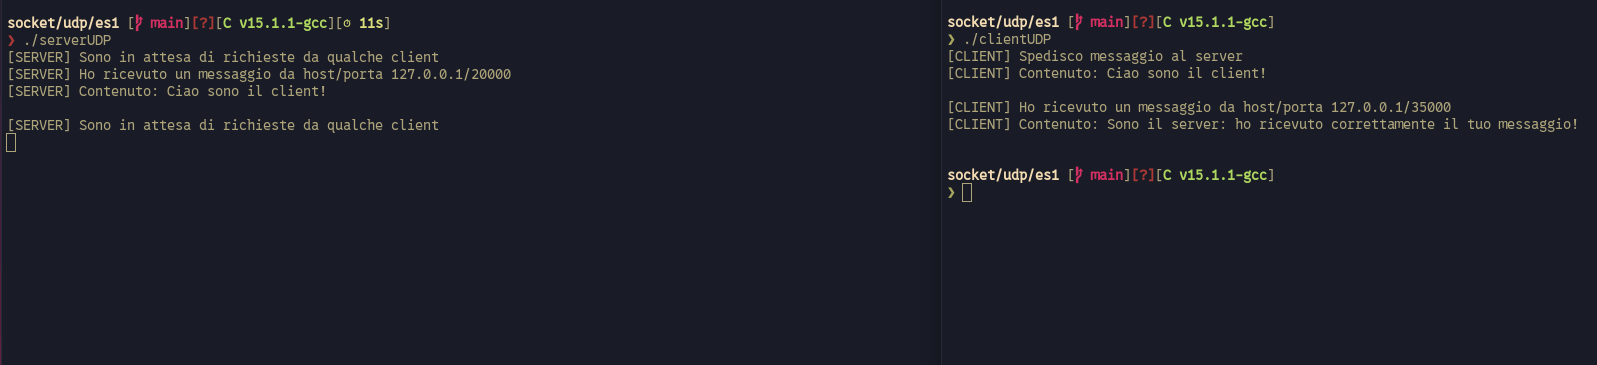
\includegraphics[width=0.7\linewidth]{server_client.png}\\
    Il server, appena avviato, resta in ascolto. Quando si avvia il client, questo invia un messaggio al server e rimane in attesa di una risposta; dopo averla ricevuta, il client termina mentre il server rimane attivo per ulteriori richieste. Invertendo l'ordine, il client invia un messaggio a un server non in ascolto (messaggio perso) e poi resta in attesa senza ricevere nulla, mentre il server avviato successivamente rimane in ascolto senza aver ricevuto richieste.

  \item \textbf{Modificare i sorgenti per mettere il server che riceve sulla porta 10000 e il client che trasmette dalla propria porta 30000.}\\
    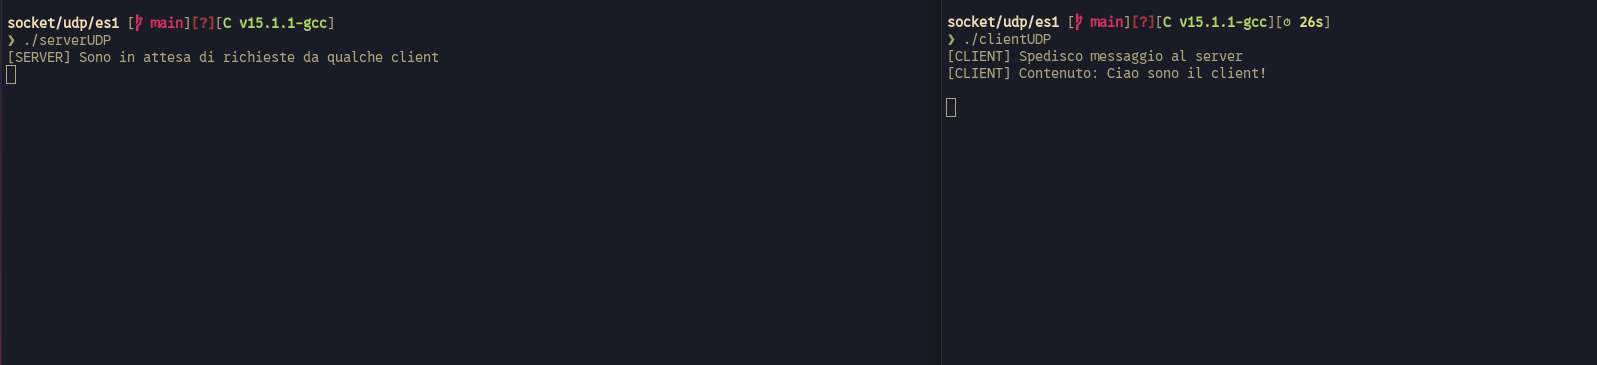
\includegraphics[width=0.7\linewidth]{cambio_porta_err.png}\\
    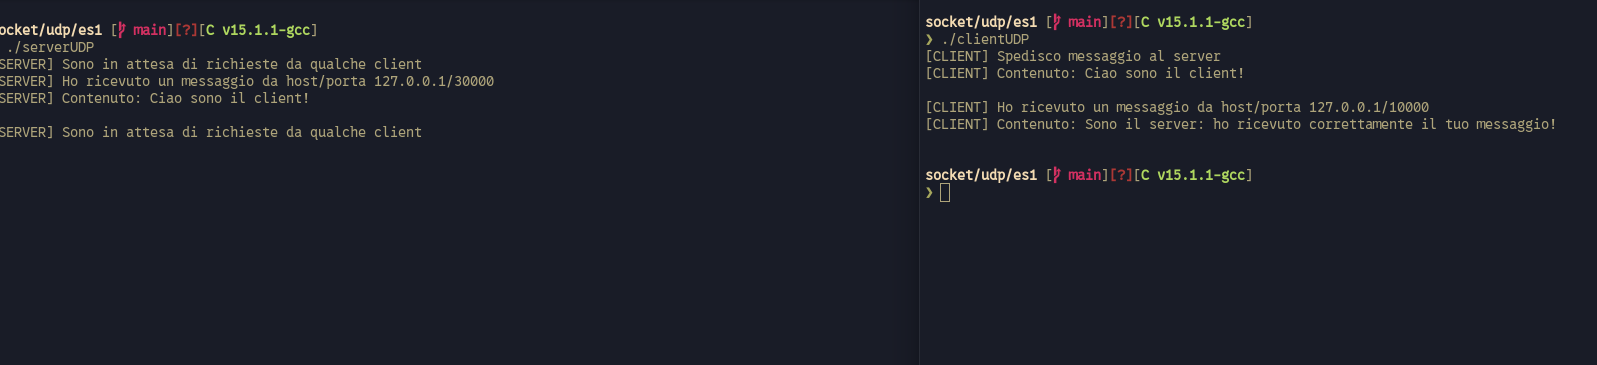
\includegraphics[width=0.7\linewidth]{cambio_porta.png}\\
    Bisogna cambiare il parametro della porta nella chiamata \texttt{createUDPInterface(10000)} sul server e \texttt{UDPSend(..., 30000)} sul client. Nella versione errata (prima immagine) la porta non è stata aggiornata; nella versione corretta (seconda immagine) la comunicazione avviene regolarmente.

  \item \textbf{Mettere il server in ascolto sulla porta 100 e osservare cosa succede.}\\
    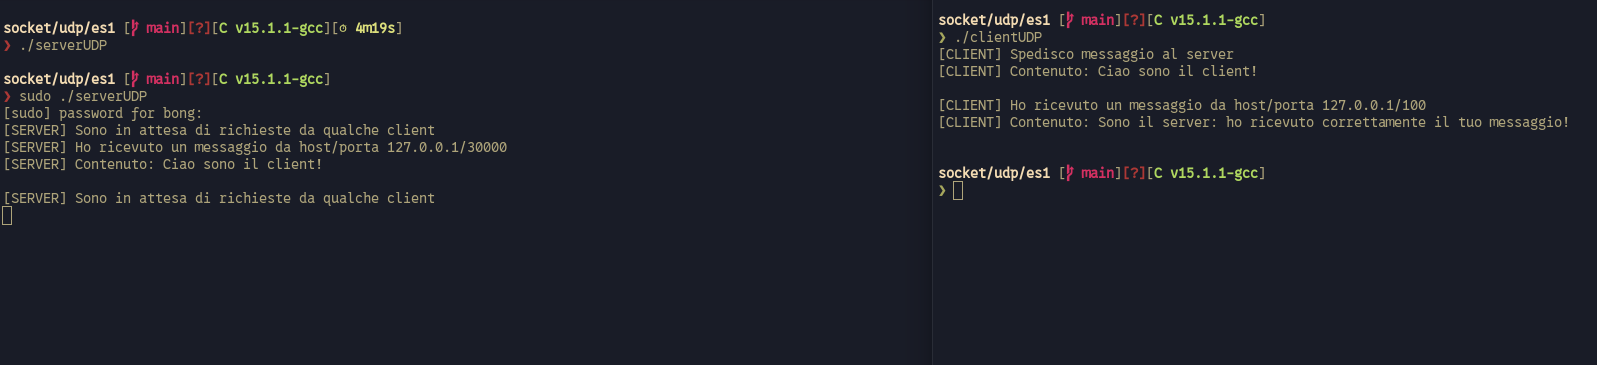
\includegraphics[width=0.7\linewidth]{cambio_porta_server.png}\\
    Dopo aver modificato la funzione di inizializzazione per usare la porta 100, il server non si avvia se eseguito senza privilegi. Le porte inferiori a 1024 sono riservate e richiedono permessi di root (sudo).

  \item \textbf{Sostituire ``127.0.0.1'' prima con ``localhost'' e poi con ``pippo'' e osservare cosa succede.}\\
    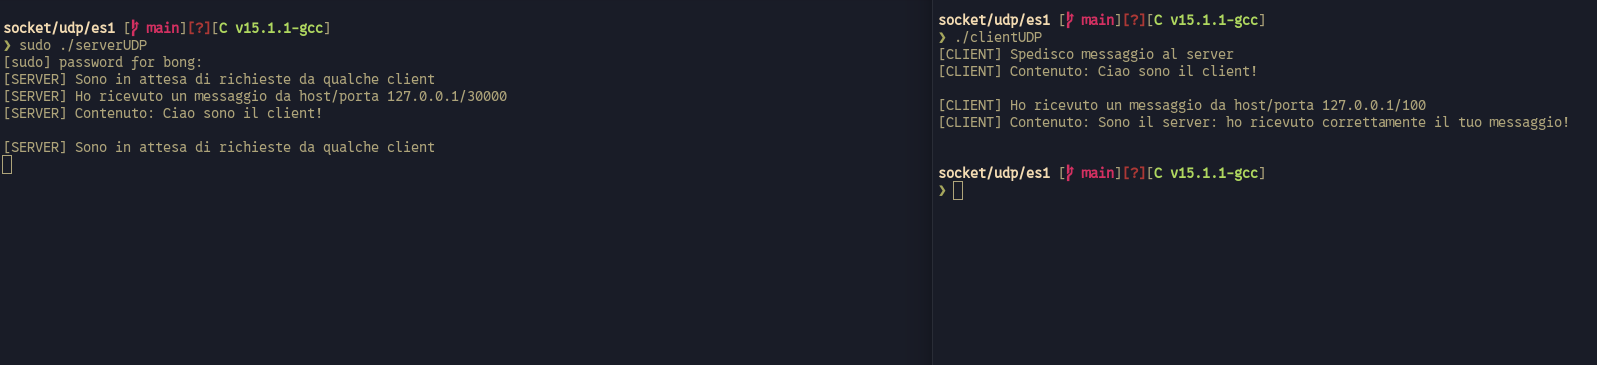
\includegraphics[width=0.45\linewidth]{ip_localhost.png}
    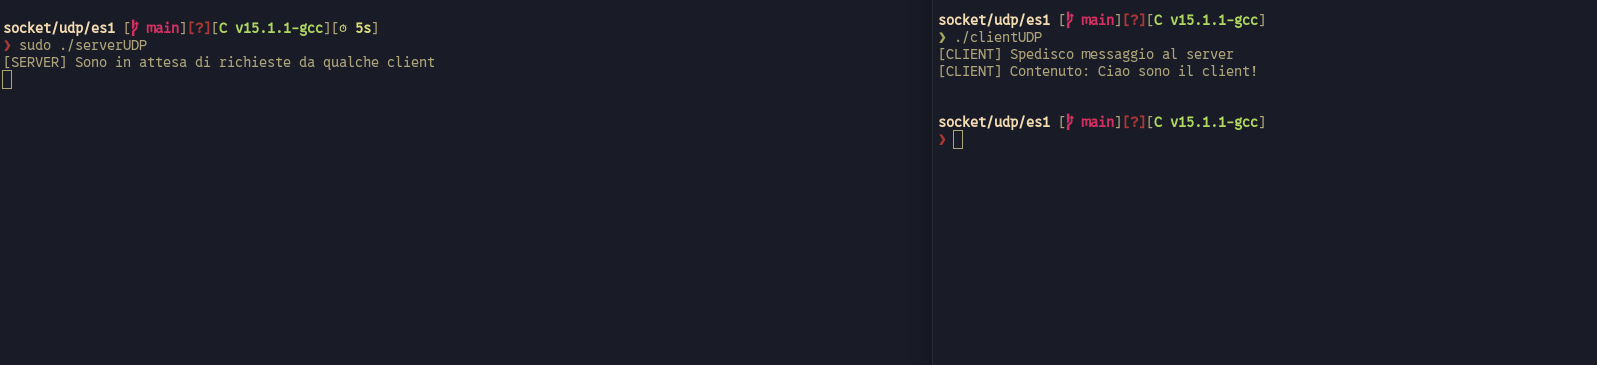
\includegraphics[width=0.45\linewidth]{ip_pippo.png}\\
    Con ``localhost'' la risoluzione DNS restituisce 127.0.0.1 e la comunicazione funziona. Con ``pippo'' non esiste alcun nome host corrispondente, quindi la chiamata fallisce.

  \item \textbf{Accordarsi per lavorare su coppie di macchine in modo che server e client siano su macchine diverse. Come bisogna modificare i sorgenti?}\\
    Bisogna trovare l'indirizzo IP della macchina che ospita il server e sostituire ``127.0.0.1'' nella chiamata \texttt{UDPSend(..., serverIP, ...)} con tale indirizzo.

  \item \textbf{Lanciare due volte il server usando due terminali. Cosa si osserva? Funzionano entrambi?}\\
    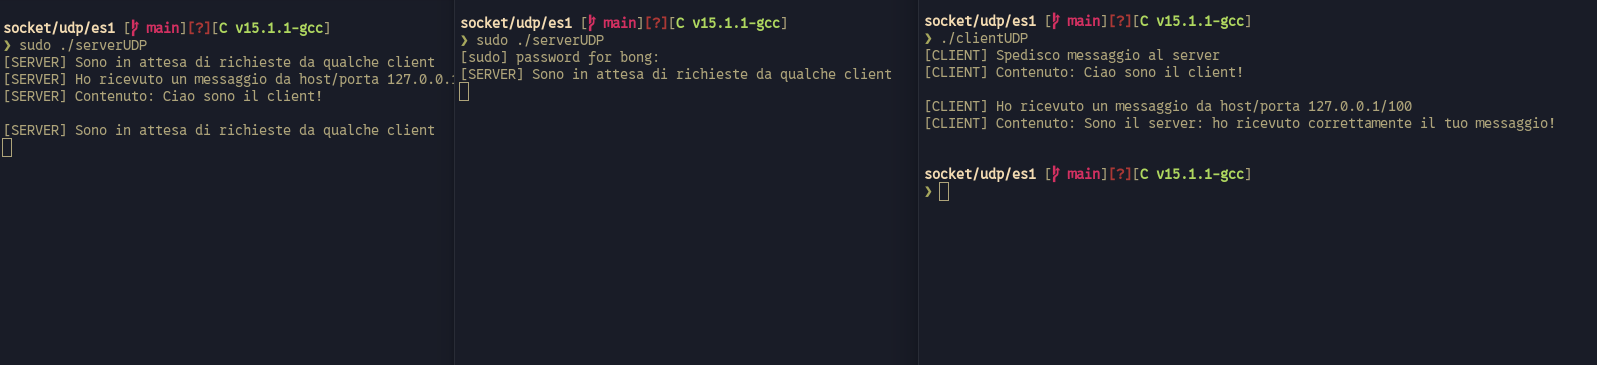
\includegraphics[width=0.7\linewidth]{due_server.png}\\
    Entrambe le istanze del server si avviano, ma solo una riceve il messaggio dal client. Le due istanze competono per la stessa porta UDP e il sistema operativo consegna il pacchetto a una sola di esse.

  \item \textbf{Modificare il server in maniera che soddisfi 5 richieste prima di terminare. E se volessi che non terminasse mai?}\\
    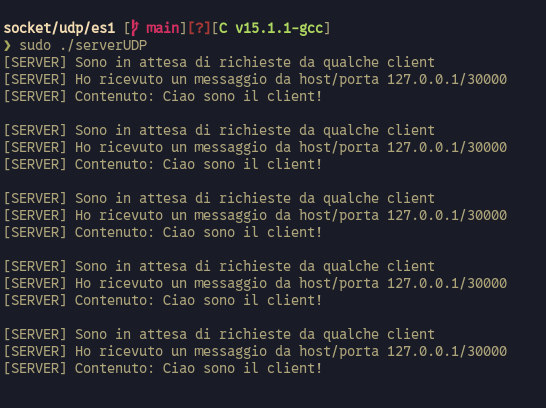
\includegraphics[width=0.7\linewidth]{cinque_client.png}\\
    Nel sorgente fornito il server è già scritto con un ciclo infinito e quindi non termina mai. Per limitarlo a 5 richieste si potrebbe introdurre un contatore e uscire dal loop dopo 5 iterazioni.
\end{enumerate}

\end{document}
